The elongation stiffness has been fit using an $\verb+fmincon.m+$, the graph and explanation is written in that specific subsection.

I have made a script in which the rotational FEM experiments can be loaded in. The top plates angle, and y-z coordinate of the end-effector is extracted from this data. This will be used as input to the IK model. We have discussed about formulating the inverse kinematics as an optimization problem to fit to the FEM data. However, it turns out that the IK solution, without optimization, already yields very satisfactory results for only a singular shape function (constant curvature approach). Therefore, optimization might not be necessary. However, I still decided to write an optimization code so also multiple shape functions can be used to approximate FEM data, it turned out the IK solver not always finds the optimum (shortest) solution. 

I have also rewritten the IK problem. Initially, I worked with an $[\theta,x,z]$ coordinate. Where $\theta$ is the orientation of the plane. However, for determining the stiffness, it might be easier to capture rotational stiffness and elongation stiffness in the modal coordinates each belonging to each degree of freedom. One that accounts for freedom in curvature and one that account for elongation.

To discuss

\begin{itemize}
       \item The IK problem has been reduced to 2 DOF. Desired end-effoctor coordinates are expressed in $x$ and $z$ not in plate rotation $\theta$ anymore. We should discuss whether or not we want to incorporate rotation aswell.
    \item The function $\verb+affine_fit.m+$ gives us a "point-on-plane", however visually this does not match that well. Maybe this is just a "note-to-self".
    \item In this approach, the real size FEM model is scaled to 1. Fed to the IK solver, and then scaled back to original length. This was a quick fix for an error when using L = 64.5 mm in the IK solver. 
    \item Have only worked slightly on the force mapping, I got an idea in my mind and I have been reading some work. But have not something usefull yet.
\end{itemize}


Three graphs are presented here below to give you a quick impression on what has been done regarding the data fitting the model.

The figure below shows the Abaqus FEM output of the undeformed (blue) bottom plane and deformed (red) top-plate. The undeformed bottom is connected to the deformed top by the red clusters of nodes. Through these red nodes the forward kinematics model should be fitted in order to map the deformation to modal coordinates $q$. The blue vector is a normal vector connected to the blue plane, the red vector is a normal vector connected to the deformed plane. An angle can be calculated between those vectors which can be used to help fitting the modal coordinates. The black point is a median of all nodes in the deformed top plate.

\begin{figure}[H]
    \centering
    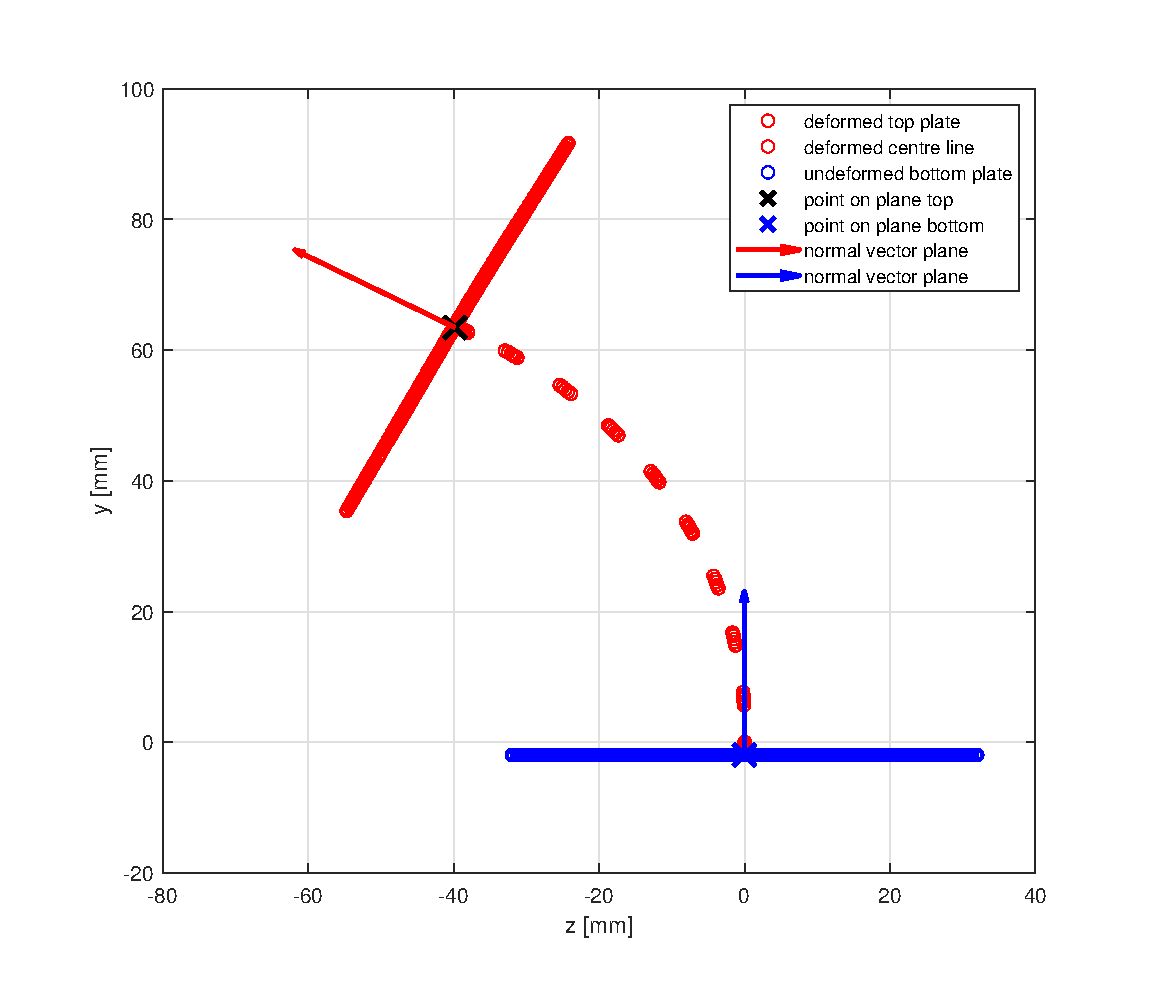
\includegraphics[width = \linewidth]{Figures/Progress/main.eps}
    \caption{Starting point, blue un deformed situation, red deformed situation}
\end{figure}

The Figure below again shows the deformed clusters nodes along the centre line. The mean of these clusters is being calculated and plotted in red. The black cross again marks a the end-effector position e.g. the point determined based on all nodes of the deformed top plate.

\begin{figure}[H]
    \centering
    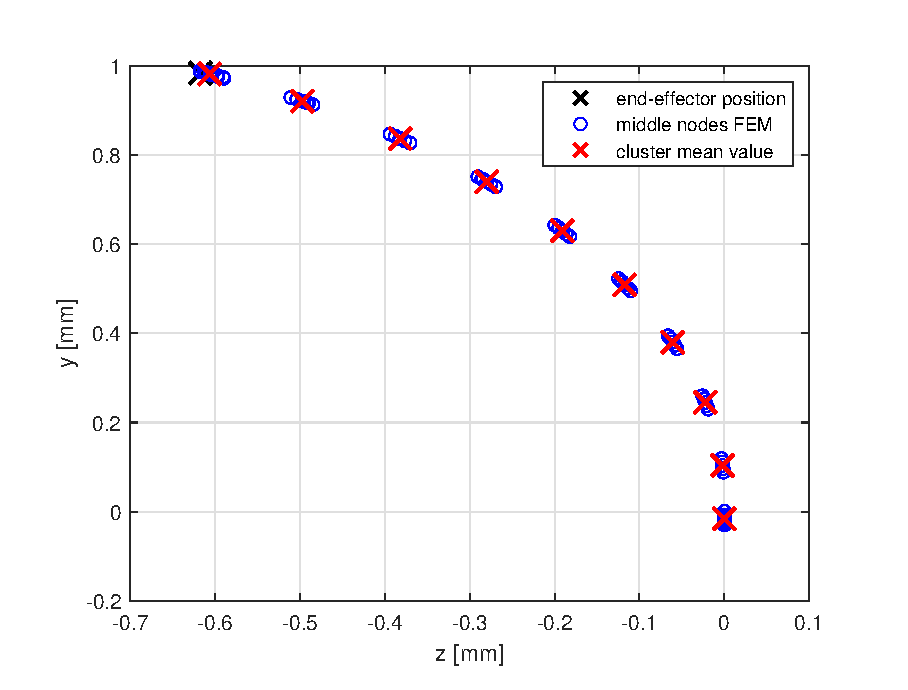
\includegraphics[width = \linewidth]{Figures/Progress/main2.eps}
    \caption{Cluster nodes are averaged, end-effector position is determined}
\end{figure}

Last figure shows an Inverse Kinematic solution to fit the deformed FEM analysis using 2 shape functions. It can be seen that by not including the angle of the top plate ($\theta$) the IK solver does not find an optimum solution and is nowhere near in describing the FEM simulation. Therefore, an optimization is carried out finding the optimal solution in fitting the FEM data. This is done by the fmincon algorithm. The objective function that is used takes into account the location of the averaged mid nodes, the arc length and the location of the end-effector.

\begin{figure}
    \centering
    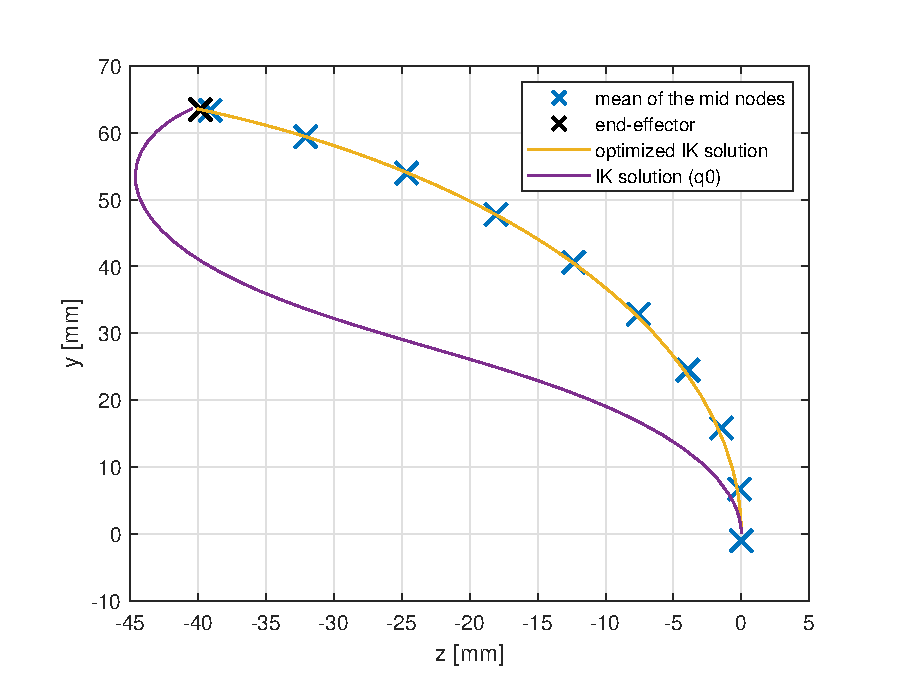
\includegraphics[width = \linewidth]{Figures/Progress/main3.eps}
    \caption{Optimization for Nmode = 2, IK solution vs optimized IK solution}

\end{figure}

